\documentclass{article}
\usepackage[T2A]{fontenc}
\usepackage[utf8]{inputenc}
\usepackage{graphicx}
\usepackage[export]{adjustbox}
\usepackage{geometry}
\usepackage{float}
\usepackage{indentfirst}


% \graphicspath{ {./img_fixed/} }

\geometry{verbose,a4paper,tmargin=2cm,bmargin=2cm,lmargin=2.5cm,rmargin=1.5cm}

% \overfullrule=2cm
\newcommand{\paragraphline}[1]{\paragraph{#1}\mbox{}\\}

\begin{document}

\begin{center}
\hfill \break
\large{МИНОБРНАУКИ РОССИИ}\\
\footnotesize{ФЕДЕРАЛЬНОЕ ГОСУДАРСТВЕННОЕ БЮДЖЕТНОЕ ОБРАЗОВАТЕЛЬНОЕ УЧРЕЖДЕНИЕ}\\ 
\footnotesize{ВЫСШЕГО ПРОФЕССИОНАЛЬНОГО ОБРАЗОВАНИЯ}\\
\small{\textbf{«ВОРОНЕЖСКИЙ ГОСУДАРСТВЕННЫЙ УНИВЕРСИТЕТ»}}\\
\hfill \break
\normalsize{Факультет компьютерных наук}\\
    \hfill \break
\normalsize{Кафедра программирования и информационных технологий}\\
\hfill\break
\hfill \break
\hfill \break
\hfill \break
\large{Отчет по предмету Архитектура информационных систем
\\1 лабораторная работа
\\Приложение для автоматизированного проведения тестирования}\\
\end{center}

\hfill \break
\hfill \break
\hfill \break
\hfill \break
\hfill \break

\begin{flushright} Вычиков Д.Д \end{flushright}
\vspace*{\fill}
\begin{center} Воронеж 2019 \end{center}
\thispagestyle{empty}
\newpage

\section{Диаграмма сущность-связь}
\begin{figure}[H]
    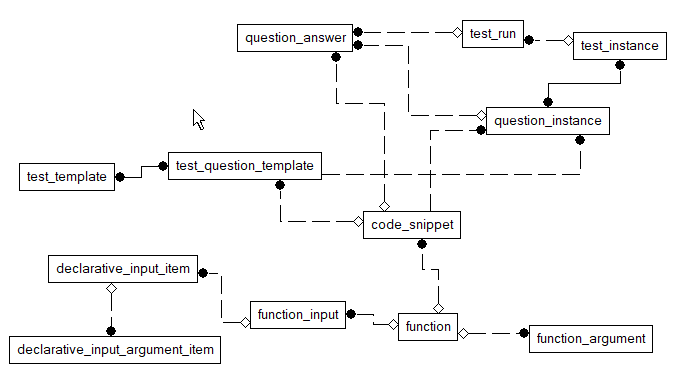
\includegraphics[width=\textwidth, center]{conceptual.png}
    \caption{Диаграмма сущность-связь}
\end{figure}
На диаграмма отображены следующие сущности:
\begin{enumerate}
    \item test\_template - Шаблон теста
    \item test\_question\_template - Шаблон вопроса
    \item code\_snippet - 
    \item test\_instance
    \item question\_instance
    \item test\_run
    \item question\_answer
    \item function
    \item function\_argument
    \item function\_input
    \item declarative\_input\_item
    \item declarative\_input\_argument\_item
\end{enumerate}
\end{document}
